% !Mode:: "TeX:UTF-8"
%此为章节二模板
%\chapter、\section、\subsection、\subsubsection分别对应一二三四级标题
\chapter{相关理论与技术介绍}\label{ch:2}
\section{姿态估计}

物体姿态估计是机器人感知中的一个关键组成部分,它使得机器人能够在非结构化环境中进行精确的操作、导航和与物体的交互。在精确授粉的机器臂应用中,准确的姿态估计对于识别花朵的位置和朝向至关重要,从而确保授粉过程的精准与高效。机械臂执行精准的手眼协调能力依赖于其估计物体姿态并适应动态环境条件的能力。为提高姿态估计的精度,可采用多种传感方式,包括基于视觉、基于深度的传感技术以及传感器融合技术。本节将概述物体姿态估计的理论基础和关键技术。

\subsection{物体姿态估计的理论基础}




物体位姿估计涉及确定物体在给定坐标系中的位置和姿态。从数学角度看,位姿估计结合了平移和旋转,可以通过不同的方法表示。
 
 \subsubsection*{(1)齐次变换矩阵}
 \FloatBarrier
 \begin{figure}[htb]
 	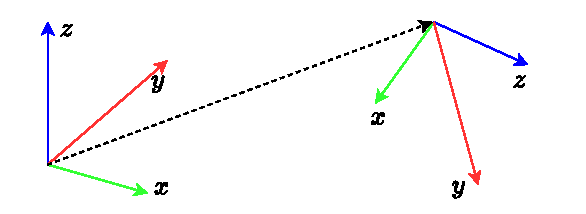
\includegraphics[width=0.7 \textwidth]{Homogeneous Transformation Matrix}
 	\caption[齐次变换矩阵]{齐次变换矩阵} % 中括号中内容为插图索引中显示内容,可在题注内容过长时使用
 	\label{fig:Homogeneous Transformation Matrix}
 \end{figure}
 
齐次变换矩阵是机器人学中广泛应用的一种表示方式,它将一个$3\times3$的旋转矩阵$R$和一个$3\times1$的平移向量$P$结合成一个$4\times4$变换矩阵$T$,如下所示:
\begin{equation}
	\label{equ:Homogeneous Transformation Matrix}
	T=
	\begin{bmatrix}
		R & P \\
		0 & 1 \\
	\end{bmatrix}=
	\begin{bmatrix}
		r_{11} & r_{12} & r_{13} & p_{1} \\
		r_{21} & r_{22} & r_{23} & p_{2} \\
		r_{31} & r_{32} & r_{33} & p_{3} \\
		0 & 0 & 0 & 1 \\
	\end{bmatrix}
\end{equation}
这种表示方法可以在统一框架中高效地组合和处理位姿,如\cref{fig:Homogeneous Transformation Matrix}所示。

 \subsubsection*{(2)欧拉角和四元数}
 
 \begin{figure}[htb]
 	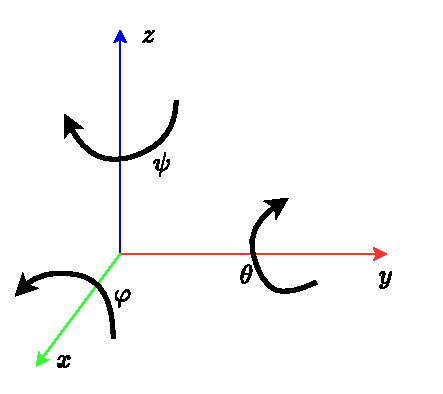
\includegraphics[width=0.43 \textwidth]{olErger.drawio}
 	\caption[欧拉角]{欧拉角} % 中括号中内容为插图索引中显示内容,可在题注内容过长时使用
 	\label{fig: olErger.drawio}
 \end{figure}
 
另一种表示姿态的方法是欧拉角,它引入了三个角度$(\phi,\theta,\psi)$,通过绕主要坐标轴的三次连续旋转来定义物体的朝向,如\cref{fig: olErger.drawio}所示,旋转矩阵$M$可以表示为三个旋转矩阵的乘积:
\begin{equation}
	\label{equ:oulEqu_1}
	M =R_{yz}(\phi)R_{zx}(\theta)R_{xy}(\psi) \\
\end{equation}
\begin{equation}
	\label{equ:oulEqu_2}
	M =
	\begin{bmatrix}
		1 & 0& 0  \\
		0 & \cos\phi & -\sin\phi \\
		0 & \sin\phi & \cos\phi  \\
	\end{bmatrix}
	\begin{bmatrix}
		\cos\theta & 0& \sin\theta  \\
		0 & 1 & 0 \\
		-\sin\theta & 0 & \cos\theta  \\
	\end{bmatrix}
	\begin{bmatrix}
		\cos\psi & -\sin\psi& 0  \\
		\sin\psi & \cos\psi & 0 \\
		0 & 0 & 1  \\
	\end{bmatrix}
\end{equation}

尽管欧拉角具有直观的优势,但它存在万向节锁死问题,即在某些情况下失去一个自由度,导致奇异性,因此不适用于连续运动应用。为了解决这一问题,四元数提供了一种更加稳定且简洁的表示方式,使用四个参数描述旋转,不会发生奇异性。它由一个标量和一个三维向量组成,表示如下:
\begin{equation}
	\label{equ:Quaternion}
	q=(w,x,y,z)
\end{equation}

$w$是标量部分,表示旋转的余弦分量,$(x,y,z)$是向量部分,表示旋转轴的正弦分量。四元数在实时应用中尤其具有优势,因为它们具有较高的计算效率和数值稳定性。

 \subsubsection*{(3)旋转向量}
 
  \begin{figure}[htbp]
 	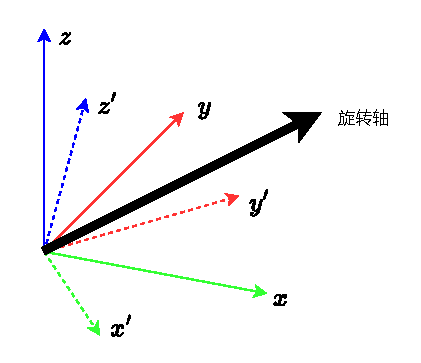
\includegraphics[width=0.43 \textwidth]{rotationVector.drawio}
 	\caption[旋转向量]{旋转向量} % 中括号中内容为插图索引中显示内容,可在题注内容过长时使用
 	\label{fig: rotationVector.drawio}
 \end{figure}
还有一种较为简洁的表示方式是旋转向量(轴-角表示),旋转向量$r$由旋转轴$v$和旋转角度$\theta$组成,定义如下:
\begin{equation}
	\label{equ:rotationVector}
	r=\theta v=(\theta v_{x},\theta v_{y},\theta v_{z})
\end{equation}

其中$v=(v_{x},v_{y},v_{z})$是旋转轴,它是一个单位向量,$\theta$ 是绕该轴旋转的角度,$r$ 是旋转向量,其方向是旋转轴,长度是旋转角度。这种表示方式通常用于优化问题中,当需要简洁但富有表达力的旋转描述时非常有用,如\cref{fig: rotationVector.drawio}所示,原坐标系$O_{xyz}$绕旋转轴旋转变换成坐标系$O_{x^{\prime}y^{\prime}z^{\prime}}$。


\subsection{坐标系与变换}
 \begin{figure}[htb]
	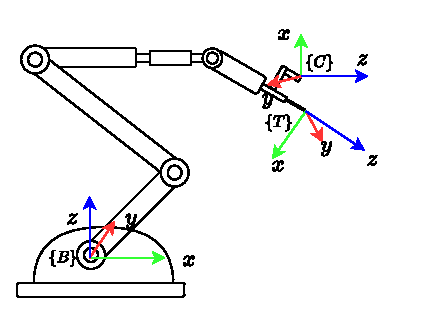
\includegraphics[width=0.6 \textwidth]{translation.drawio}
	\caption[机械臂中各个坐标系]{机械臂中各个坐标系} % 中括号中内容为插图索引中显示内容,可在题注内容过长时使用
	\label{fig:translation.drawio}
\end{figure}

在机器人视觉系统中,多个坐标系的精确变换至关重要,包括机器人基座坐标系(Base, \{B\})、末端TCP坐标系(Tool Center Point, TCP, \{T\})、相机坐标系(Camera, \{C\}),以及世界坐标系(World, \{W\}),如\cref{fig:translation.drawio}所示。这些坐标系之间的相互转换是保证机器人精准感知环境、执行任务的关键因素。特别是在动态任务中,坐标精度的误差可能直接影响机器人操作的成功率。因此,采用合理的运动学建模和手眼标定技术,建立精确的坐标转换关系,对于提升机器人系统的操作精度和稳定性具有重要意义。

\subsubsection*{(1)机械臂基座坐标系 }
机器人基座坐标系 \{B\} 作为整个机械臂系统的全局参考系,其原点通常位于机械臂的底座中心,$Z$轴垂直向上,$X$轴沿机械臂初始运动方向。所有关节和末端执行器的位置均相对于该坐标系进行定义。
\subsubsection*{(2)末端TCP 坐标系  }
TCP 坐标系\{T\} 由末端执行器(如夹爪)的工作点决定,通常不与机械臂法兰坐标系重合,而是存在一定的偏移量。其位置和姿态由机器人运动学方程(基于 Denavit-Hartenberg, DH 参数法)计算得出,即:
\begin{equation}
	\label{equ:coordinate_b_t}
	T^{B}_{T}=T^{B}_{J} \cdot T^{J}_{T} 
\end{equation}

其中,$T^{B}_{T} $为基座到机械臂关节的变换矩阵,$JT^{J}_{T}$为机械臂末端的工具偏移矩阵。通过该变换,可以从基座坐标系计算出 TCP 的位姿。
\subsubsection*{(3)相机坐标系 }
相机坐标系\{C\}由安装在机械臂上的视觉传感器(如RGB-D相机)定义,其原点位于相机光心,Z 轴朝向相机视线方向,X 轴向右,Y 轴向下。为了使相机与末端执行器协同工作,必须进行手眼标定(Hand-Eye Calibration),以求得相机与 TCP 之间的空间变换矩阵$T^{T}_{C}$。

\subsubsection*{(4)世界坐标系 }
在许多视觉任务中,机器人需要将检测到的目标点从相机坐标系 $\{C\}$ 映射到世界坐标系 $\{W\}$,这通常通过外部标定方法(如 AprilTag 或棋盘标定)获得变换矩阵 $T^{W}_{C}$。最终,目标点的世界坐标可以通过以下公式计算:
\begin{equation}
	\label{equ:coordinate_w_c}
	P_{W}=T^{W}_{C} \cdot P_{C} 
\end{equation}

其中,$P_{C} $为相机坐标系中的目标点,$P_{W}$为世界坐标系中的目标点。

\subsubsection*{(5)机械臂多坐标系转换的数学描述 }
2. 机械臂多坐标系转换的数学描述
各坐标系之间的变换通常采用齐次变换矩阵(Homogeneous Transformation Matrix),其形式为:
\begin{equation}
	\label{equ:coordinate_base}
	T^{A}_{B} =
	\begin{bmatrix}
		R_{3 \times 3} & t_{3\times 1}  \\
		0_{1 \times 3} & 1\\
	\end{bmatrix}
\end{equation}


其中$R_{3 \times 3}$为3$\times$3旋转矩阵,描述坐标系的方向变换; $t_{3 \times 1}$为3$\times$1平移向量,描述坐标系的位移变换。综合考虑所有坐标系的变换关系,目标点在基座坐标系中的表示可通过如下公式计算:

\begin{equation}
	\label{equ:coordinate_base_2}
	P_{B} = T^{B}_{T} \cdot T^{T}_{C} \cdot P_{C}
\end{equation}

这表明,若相机检测到某目标点$P_{C}$,可通过末端的手眼标定矩阵$T^{T}_{C}$以及机械臂运动学矩阵$T^{B}_{T}$进行转换,从而得到该目标点在基座坐标系中的位置。


\subsection{物体姿态估计技术}
\subsubsection{基于特征的姿态估计}
基于特征的物体姿态估计方法专注于检测和匹配图像中的显著特征。这些特征作为地标,帮助识别和定位三维空间中的物体。这些经典方法通常用于2D到3D的姿态估计任务,其中通过图像关键点与3D模型点的特征匹配来计算物体在相机坐标系中的姿态。

 \subsubsection*{(1)尺度不变特征变换}
尺度不变特征变换(SIFT) 在三维物体位姿估计任务中,SIFT算法通常用于从单张或多张二维图像中提取稳定的特征点,然后通过匹配这些特征点来推测物体在三维空间中的位置和朝向。

首先,通过从不同视角下拍摄的二维图像中提取SIFT特征点,算法能够在图像中找到具有显著差异和鲁棒性的局部特征。对于每个关键点,SIFT算法会生成一个包含局部图像梯度信息的描述符,确保在光照、旋转、尺度变化等变换下依然能准确地匹配相同的特征点。然后,使用这些匹配的特征点,结合相机的内外参(如相机的焦距和位置),通过几何计算方法(例如PNP算法)来估计物体的位姿。

在实际应用中,SIFT常与其他算法如PNP(Perspective-n-Point)和RANSAC结合使用,以增强位姿估计的准确性和鲁棒性。PNP算法用于通过一组已知3D点与其对应的2D投影点来估计相机的位置和朝向,而RANSAC则用于在特征匹配过程中剔除错误匹配点,从而提升结果的稳定性和准确性。

SIFT在三维物体位姿估计中的一个典型应用是增强现实(AR)。在增强现实应用中,SIFT被用来实时追踪物体的位置和姿态,并将虚拟信息叠加到实际场景中。这要求对物体的三维模型有准确的先验信息,并通过特征匹配来持续调整位姿估计,以确保虚拟物体能够正确地与现实世界中的物体对齐。

此外,SIFT也被广泛应用于3D重建任务中。在多视角的图像中提取到的特征点可以用于通过三角测量计算三维点的空间位置,进而重建出三维物体或场景。该过程中的特征匹配是实现精确重建的关键步骤,而SIFT提供了在不同视角下稳定且独特的特征描述符,极大地提高了匹配的成功率。
 \subsubsection*{(2)加速稳健特征}
SURF(加速稳健特征,Speeded-Up Robust Features) 是一种用于图像特征检测与描述的算法,旨在提高SIFT算法的计算效率,同时保持其稳健性。SURF算法由Bay等人于2006年提出,并在多个计算机视觉任务中广泛应用,如图像匹配、目标识别、三维重建和图像拼接等。与SIFT类似,SURF能够有效地检测到尺度、旋转和光照变化下稳定的特征点,但通过改进计算方法,显著提高了速度。

SURF的核心改进之一是采用Hessian矩阵来进行尺度空间中的特征点检测。通过近似计算Hessian矩阵,Hessian矩阵的形式如下:
\begin{equation}
	\label{equ:Hessian}
	H(x,\sigma) =
	\begin{bmatrix}
		D_{xx}(x,\sigma) & D_{xy}(x,\sigma)  \\
		D_{xy}(x,\sigma)  & D_{yy}(x,\sigma) \\
	\end{bmatrix}
\end{equation}

其中$D_{xx}(x,\sigma)$ ,$D_{xy}(x,\sigma)$ ,$D_{yy}(x,\sigma)$ 是图像的二阶偏导数,表示图像在各方向的曲率。Hessian矩阵的特征值能够反映图像中局部区域的强度变化,从而识别出重要的特征点。

SURF能够在不同尺度下快速检测到图像中的显著特征点。此外,SURF通过引入积分图的加速技术,使得图像梯度的计算更加高效,从而降低了计算复杂度,相较于SIFT在处理速度上具有显著优势。

为了实现旋转不变性,SURF为每个特征点分配一个主方向,该方向基于关键点邻域内的梯度方向进行计算。SURF的特征描述符基于Haar小波响应,通过计算关键点邻域内的局部梯度来生成描述符。这些描述符能够高效地描述图像的局部结构,并且在光照、旋转和尺度变化下保持不变性。

SURF在计算效率上优于SIFT,是一个在许多计算机视觉任务中广泛应用的强大工具,尤其是在需要快速特征提取和匹配的场景中,如全景拼接、实时物体追踪和三维重建等。
 \subsubsection*{(3)Oriented FAST and Rotated BRIEF}
ORB(Oriented FAST and Rotated BRIEF)是一种结合了FAST角点检测和BRIEF描述符的特征点检测与描述算法,主要用于计算机视觉中的特征匹配和图像配准。它由Ethan Rublee等人于2011年提出,旨在提高传统方法在旋转不变性和计算效率上的性能。ORB不仅具备较高的鲁棒性,还能在实时应用中保持较快的运行速度,因此被广泛应用于诸如物体识别、图像拼接和机器人定位等领域。

ORB的核心思想是首先使用FAST(Features from Accelerated Segment Test)角点检测器来检测图像中的角点。FAST是一个高效的角点检测方法,通过分析像素点周围区域的亮度变化来确定角点的存在。与传统的Harris角点检测器相比,FAST具有更快的计算速度,适合于实时处理。但仅使用FAST检测到的角点并不足以解决旋转和尺度变化的问题,因此ORB引入了对角点的方向性分析,以实现对旋转变化的鲁棒性。

为了进一步提高描述符的质量和匹配的准确性,ORB采用了BRIEF(Binary Robust Independent Elementary Features)描述符。BRIEF通过比较特征点邻域内像素对的亮度值来生成二进制字符串,用以描述特征点周围的局部图像信息。这使得描述符具有非常高的计算效率,并且容易存储。然而,BRIEF本身对旋转不具备鲁棒性,因此ORB在生成BRIEF描述符之前,会先为每个角点计算一个主方向,使得生成的描述符在旋转后的图像中仍能保持一致。

尽管ORB并不像SIFT或SURF那样直接支持尺度不变性,但通过图像金字塔结构,ORB可以在不同尺度下检测和描述特征点,从而实现一定程度的尺度不变性。这使得ORB在处理图像中的尺度变化时仍然能够保持较好的表现。此外,ORB具有较强的抗噪声能力,能够在低质量或含有噪声的图像中进行有效的特征匹配和追踪。

\subsubsection{基于深度学习的方法}
与传统方法不同,基于深度学习的方法利用大规模数据集和卷积神经网络(CNN)直接从原始图像数据中估算物体姿态,从而省略了显式的特征提取。这些方法能够有效处理复杂场景,包括遮挡和视角变化,传统方法可能无法应对这些情况。以下是一些在物体姿态估计中突出的深度学习方法:
 \subsubsection*{(1)PoseNet}
PoseNet是一个基于CNN的模型,能够直接从单张图像中估算物体的六维姿态(位置和朝向)。它旨在高效地用于实时应用,如移动和机器人系统。PoseNet使用一个预训练的网络,能够回归物体的平移(位置)和旋转(朝向)。该模型对各种条件具有鲁棒性,包括光照变化、遮挡和尺度变化。PoseNet在大规模已知姿态物体的数据集上进行训练,并能够通过根据图像特征调整参数来推广到新的场景。
 \subsubsection*{(2)DenseFusion}
DenseFusion采用了一种混合方法,通过结合CNN和几何推理来提高姿态估计的精度。该方法融合了RGB和深度数据以提取稠密的逐点特征,从而更好地处理遮挡和杂乱环境。DenseFusion首先从RGB图像和深度图中提取特征,然后在点级别融合这些特征,生成更丰富的物体表示。通过使用这两种模态,DenseFusion在6D姿态估计任务中表现出色,尤其在复杂的现实环境中,纯RGB方法可能会失效。
\subsubsection*{(3)PVNet}
PVNet采用基于关键点的方法来估算物体的姿态。该模型被训练用于检测图像中物体上的关键点,然后利用这些关键点回归六维姿态。与PoseNet直接回归姿态不同,PVNet首先预测关键点,然后通过统计投票机制来确定姿态。这种方法特别适用于遮挡情况,因为缺失的关键点可以通过投票机制处理。PVNet特别适用于具有对称结构的物体,如圆柱形或球形物体,而这些物体对依赖特征匹配的方法来说可能是挑战。
\subsubsection{基于深度的姿态估计}
基于深度的方法依赖于使用3D信息来更准确地估算物体姿态。通过利用RGB-D相机或LiDAR等深度传感器,这些技术能够在复杂的现实场景中提供更稳健的姿态估计解决方案。
\subsubsection{传感器融合技术}
为了提高姿态估计的鲁棒性,传感器融合技术结合了来自多种传感器的信息,如视觉相机、深度传感器和惯性测量单元(IMU)。这些方法通过弥补单一传感器的局限性,提升了性能。
\subsection{精确授粉中的应用}
在机器人授粉中,精确的物体姿态估计对于识别和与花朵的交互至关重要。准确的姿态估计可以实现花朵的检测和定位,使机器人臂能够以最小误差接近目标。此外,动态姿态估计能够适应风等环境因素引起的花朵运动,确保机器人能够实时适应。基于估算姿态的轨迹规划优化了机器人臂的运动,提高了效率并减少了不必要的能量消耗。实时更新姿态的能力增强了系统的适应性和授粉任务的整体成功率。

\section{机械臂运动规划}
运动规划是机器人学中的一项关键任务,特别是对于介尺度机械臂,它们被设计用于执行精确和细致的运动。这些机器人臂广泛应用于需要高精度的领域,如精准授粉、外科机器人和微组装等。运动规划的目标是生成一条轨迹,使机器人臂能够从初始位置移动到目标位置,同时避开障碍物并优化运动效率。在环境要求机器人臂必须适应动态条件时,运动规划任务会变得更加复杂,使得适应性成为规划过程的关键因素。
传统的运动规划方法,如插值法,在结构化环境中有效,提供了平滑和高效的路径。然而,随着机器人任务的复杂性增加,特别是在非结构化环境中,新的技术如深度学习逐渐成为有价值的工具。这些方法使机器人臂能够通过从环境反馈和传感数据中学习,自主地调整到新的情境中。本文讨论了基于传统插值法的方法和现代深度学习方法,并强调了每种方法在解决机器人运动规划挑战,特别是精准授粉任务中的贡献。
在执行精密操作时,介尺度机械臂面临几项关键挑战。包括:
1.	精度与准确性:高精度对于执行如花粉传播等细致任务至关重要,因为即便是微小的运动偏差也可能导致失败。机器人臂必须执行高精度的运动,通常需要达到亚毫米级的精度,以避免损坏易碎的物体或组件。
2.	动态环境:机器人臂必须在动态环境中工作,障碍物或物体可能会不可预测地移动,这要求机器人臂实时调整其轨迹。在某些应用中,环境可能还包括变化的光照条件或杂乱的场景,进一步增加了运动规划的难度。
3.	有限的工作空间与障碍物:许多机器人臂在空间有限的环境中操作,必须高效地避免碰撞。路径规划必须考虑到障碍物以及与其他物体或机器人系统的潜在干扰,确保机器人臂在有限的工作空间内安全有效地移动。
当这些因素相互结合时,运动规划的复杂性增加,因此需要结合传统方法与深度学习技术,以达到最佳性能。



\subsection{传统运动规划方法}

在实际应用中,插值方法被广泛用于路径生成和轨迹规划。例如,在精准授粉中,机器人臂需要沿着预定义路径运动,同时避开障碍物并减少对脆弱花朵的影响。通过使用三次或五次样条插值,机器人臂可以生成最小化突然运动的轨迹,确保路径点之间的平稳过渡。
插值方法使机器人能够高效地跟随复杂路径,无论是在关节角度还是末端执行器的位置之间进行插值。在授粉任务中,机器人臂必须从一朵花移动到另一朵花,运动的平滑性至关重要,以避免对花朵造成损害。使用三次和五次样条插值确保机器人可以平稳地从一个位置到另一个位置,调整花朵的朝向等环境变化。
插值方法还帮助优化时间和能量消耗。通过生成优化路径,机器人臂可以减少不必要的运动,从而提高任务效率。在精准授粉的背景下,减少运动时间对于提高产量和提升系统性能非常重要。
插值法长期以来一直是机器人臂运动规划的核心技术。它通过计算预定义路径点之间的中间点,生成机器人臂的平滑路径。几种插值方法在实践中被广泛应用:

\subsubsection{线性插值(Lerp)}
线性插值,也叫Lerp,是最简单的插值形式,其中两个点之间的轨迹为一条直线。它在计算上高效,易于实现。然而,对于需要平滑过渡的复杂任务,线性插值通常过于简单。例如,当机器人在两个点之间改变朝向时,线性插值可能会导致抖动,这在精密任务如授粉中是不希望发生的。
\subsubsection{三次样条插值}
为了克服线性插值的局限性,常常采用三次样条插值。三次样条是分段多项式,在每一对路径点之间拟合三次多项式。该方法确保在路径点处位置和速度是连续的,从而减少运动中的突然跳跃。
三次样条插值方法通过解一个方程组来强制在路径点处保持平滑。通过这种方式得到的路径,确保了位置和速度的平稳过渡,使其在精密操作中更加适用,在这些任务中需要最小化突加速度(即加速度的变化率)。在如装配或授粉这样的任务中,三次样条确保机器人臂以平滑且可预测的方式运动。
\subsubsection{五次样条插值}
对于要求更平滑运动的任务,采用五次样条插值。五次样条扩展了三次样条,使用更高阶的多项式,特别确保了位置、速度和加速度的连续性。五次样条插值最小化了突加速度,使其非常适合高精度应用。在执行如花粉传播等精密任务时,机器人臂必须平滑地调整轨迹,避免突然的加速度,以防损坏易碎的物体。

\subsection{深度学习方法}
尽管传统的插值方法在控制环境中有效,但深度学习在解决更复杂的动态运动规划挑战中越来越受到关注。深度学习技术,特别是虽然传统的插值方法在结构化环境中很有用,但深度学习技术在解决复杂运动规划问题,特别是在动态或非结构化环境中,越来越受到重视。深度学习使机器人臂能够从传感器数据中学习,从而提高其在实时环境中的适应性和决策能力。
\subsubsection{强化学习(RL)}
强化学习(RL)是深度学习在机器人运动规划中的一项重要技术。在RL中,机器人臂通过与环境互动来学习执行任务。机器人通过奖励和惩罚的反馈来指导学习过程。随着时间的推移,机器人形成最优策略,以最大化其累计奖励。
例如,在精准授粉任务中,RL可以用来教机器人臂如何根据传感器反馈,如相机图像或力传感器,避开损坏。机器人通过成功授粉得到正反馈,通过扰动得到负反馈。通过反复试验,机器人臂学习到最优策略,以最小化错误并最大化效率。
强化学习技术,如深度Q网络(DQNs)和近端策略优化(PPO),可以用来训练机器人臂实时执行复杂任务。这些技术使机器人臂能够通过调整其策略,以适应新的情境并进行优化。
\subsubsection{卷积神经网络(CNNs}
在动态环境中的运动规划中,机器人对其环境的感知和理解至关重要。卷积神经网络(CNNs)在处理视觉数据方面表现优异,如图像或点云数据,因此它们在进行物体检测和环境交互等任务时非常适用。
例如,执行精准授粉的介尺度机械臂可以依赖CNN来检测花朵的位置并识别工作空间中的障碍物。CNN处理来自机器人相机或激光雷达(LIDAR)传感器的输入,进行对象的分割和分类。基于这些视觉信息,机器人臂可以调整路径,以避开障碍物、检测花朵的位置并优化授粉方法。
CNN通过大量的图像数据进行训练,使机器人能够在不同情境下进行泛化,适应光照、花朵形状和朝向的变化。这种实时处理复杂感知数据的能力是深度学习相对于传统插值方法的一大优势。


\subsection{混合方法}
深度学习与传统运动规划方法的混合方式提供了两者的优点。在这种方法中,深度学习模型处理动态环境适应,而传统的插值技术则确保机器人在关键路径点之间进行平稳有效的运动。例如,CNN可以用于识别物体和障碍物,而插值方法如五次样条插值则确保机器人在从一个点到下一个点时平滑运动,最小化突加速度并提高精度。
这种混合方法在需要高适应性和高精度的任务中非常有用,如精准授粉或微组装,其中机器人臂必须在动态环境中导航,同时保持高度精确。

\subsection{结论}
介尺度机械臂的运动规划是一个多方面的挑战,需要结合传统方法与先进的深度学习技术。插值方法继续为在控制环境中生成平稳、无碰撞的运动提供有效解决方案,而深度学习增强了机器人在动态和无结构环境中的适应能力。通过将这两种方法结合起来,混合方案为在复杂、动态环境中执行高精度任务提供了有力的支持。随着技术的发展,深度学习与传统规划算法的结合将推动下一代机器人系统的发展,使它们能够以更高的效率和自主性执行复杂的精密任务。




